%!TEX program = xelatex
\documentclass[tikz]{standalone}
\usepackage{pgfplots}
\usepgfplotslibrary{patchplots,colormaps,colorbrewer}
\pgfplotsset{compat=1.18}
\usepackage{xcolor}

\begin{document}
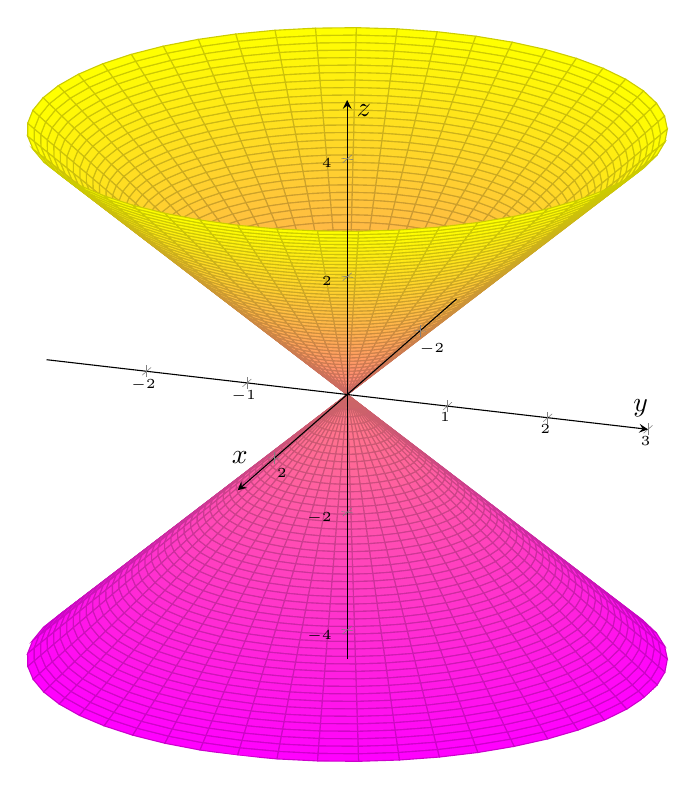
\begin{tikzpicture}
    \begin{axis}[
        tick label style={font=\tiny}, 
        view={110}{20}, 
        axis lines=center,
        xlabel={$x$}, ylabel={$y$}, zlabel={$z$},
        xmax=3, ymax=3, zmax=5,
        width=12cm, 
        height=12cm,
        axis on top
    ]
        \addplot3 [
            colormap/spring, 
            surf, 
            z buffer=sort, 
            samples=50,  
            domain=0:3, 
            y domain=0:2*pi
        ] ({x*cos(deg(y))}, {x*sin(deg(y))}, {1.5*x});
        
        \addplot3 [
            colormap/spring, 
            surf, 
            z buffer=sort, 
            samples=50,  
            domain=0:3, 
            y domain=0:2*pi
        ] ({x*cos(deg(y))}, {x*sin(deg(y))}, {-1.5*x});
    \end{axis}
\end{tikzpicture}
\end{document}